
\subsection{Overview}
In response to the pilot results, we reconsider the data collection pipeline to reduce the uncertainty around collecting drawings that illustrate the prompts and textual descriptions well-aligned with each step in the drawing. Firstly, in order to alleviate the burden of drawing from the annotators, we examined existing sketch datasets, and information regarding the advantages and disadvantages are shown in Table v2.datasets.1.   
[Table v2.datasets.1: pros and cons, stats of different sketch datasets]

Between Sketch Perceptual Grouping (SPG) and SketchSeg, both containing annotaiton for semantically meaningful parts in sketches, SPG annotates for QuickDraw sketches while SketchSeg collects its own sketches. We picked SPG, since it will be easier in the future to extend our datasets given the large QuickDraw reservoir of sketches. Moreover, SketchSeg dataset contains a \textit{fourleg} category that includes many different kinds of animals, such as horse, sheep, and cow, but the QuickDraw categories are more fine-grained, so form a model learning perspective, SPG will also be more generalizable. Therefore, to combine our previous goal, collecting sketches that illustrate certain \textit{adjective}$\times$\textit{noun} prompts, we decided to provide annotators with the sketches from QuickDraw and ask them to annotate for each semantically meaningful part provided in the SPG Dataset. 

In order to avoid dealing with discrepancies between performance of fellow graduate students and that of the turkers, we deployed a short pilot test of the new version and identified the suitable format and areas that need written requirement for the turkers to avoid these mistakes.   
Therefore, the transformation of the task format is driven by mistakes we have seen during the pilot trials. 

\subsubsection{Main Task}
In Figure \ref{v2.main_task.1}, we show the transformation from our first pilot of version to the final task that is deployed to collect the entire dataset. 
Overall, we used non-gray colors to highlight the parts in the sketch that we want annotations, another design to help with annotation speed. 
For simplicity, we restricts the annotations from whole sentences (Figure \ref{v2.main_task.1.a}) to only adjective phrases (Figure \ref{v2.main_task.1.b}, \ref{v2.main_task.1.c}, \ref{v2.main_task.1.d}). The benefit of juxtaposing two sketches and simultaneous annotate for two sketches is that annotators are implicitly encouraged to provide descriptions that identify features of the objects that differentiate the two sketches. This method is also proposed to facilitate the annotation process and to take less time, since it is easier to differentiate and perform a contrasting task than to generate descriptions from a single sketch. 
At the beginning, we explicitly mention that the goal of the task is to describe the differences between the objects in the sketches (\textit{Describe differences} in \ref{v2.main_task.1.a} and \textit{Compared to Sketch 1/2} in \ref{v2.main_task.1.b}), and we received many annotations that contain comparative and superlatives, so we eventually only have a blank without any introductory phrases to overly emphasize that the goal of the tasks is to create a dataset of contrastive pairs of descriptions, and the juxtaposition is meant only as a mental hint to ease annotation.

\begin{figure*}[ht!]
\begin{subfigure}{\textwidth}
  \centering
  % include first image
  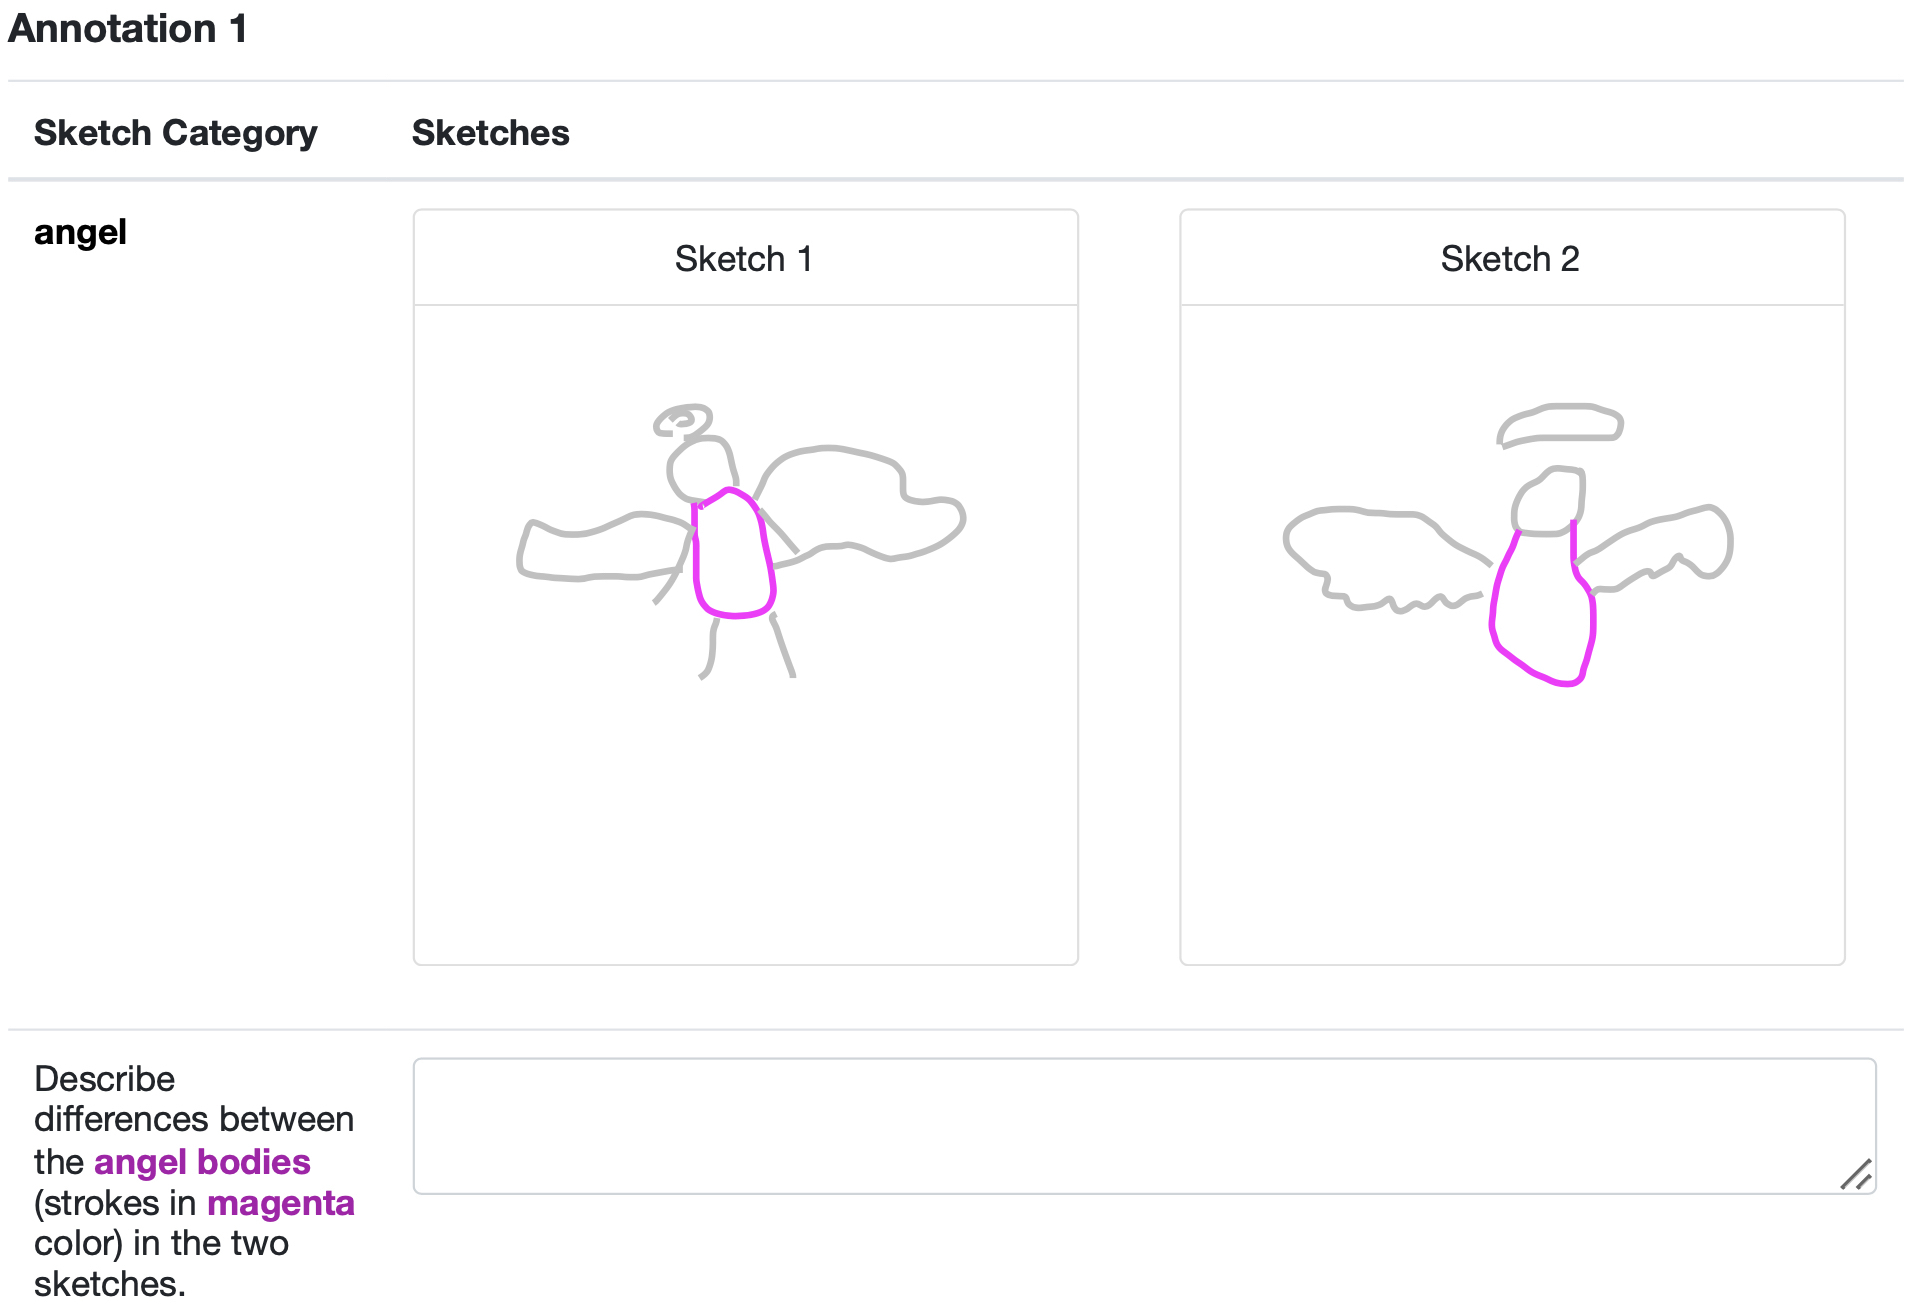
\includegraphics[width=.8\linewidth]{data_collection/pilot_02_01_annotation_1.png}  
  \caption{Design of main task for first pilot.}
  \label{v2.main_task.1.a}
\end{subfigure}
\newline
\begin{subfigure}{\textwidth}
  \centering
  % include third image
  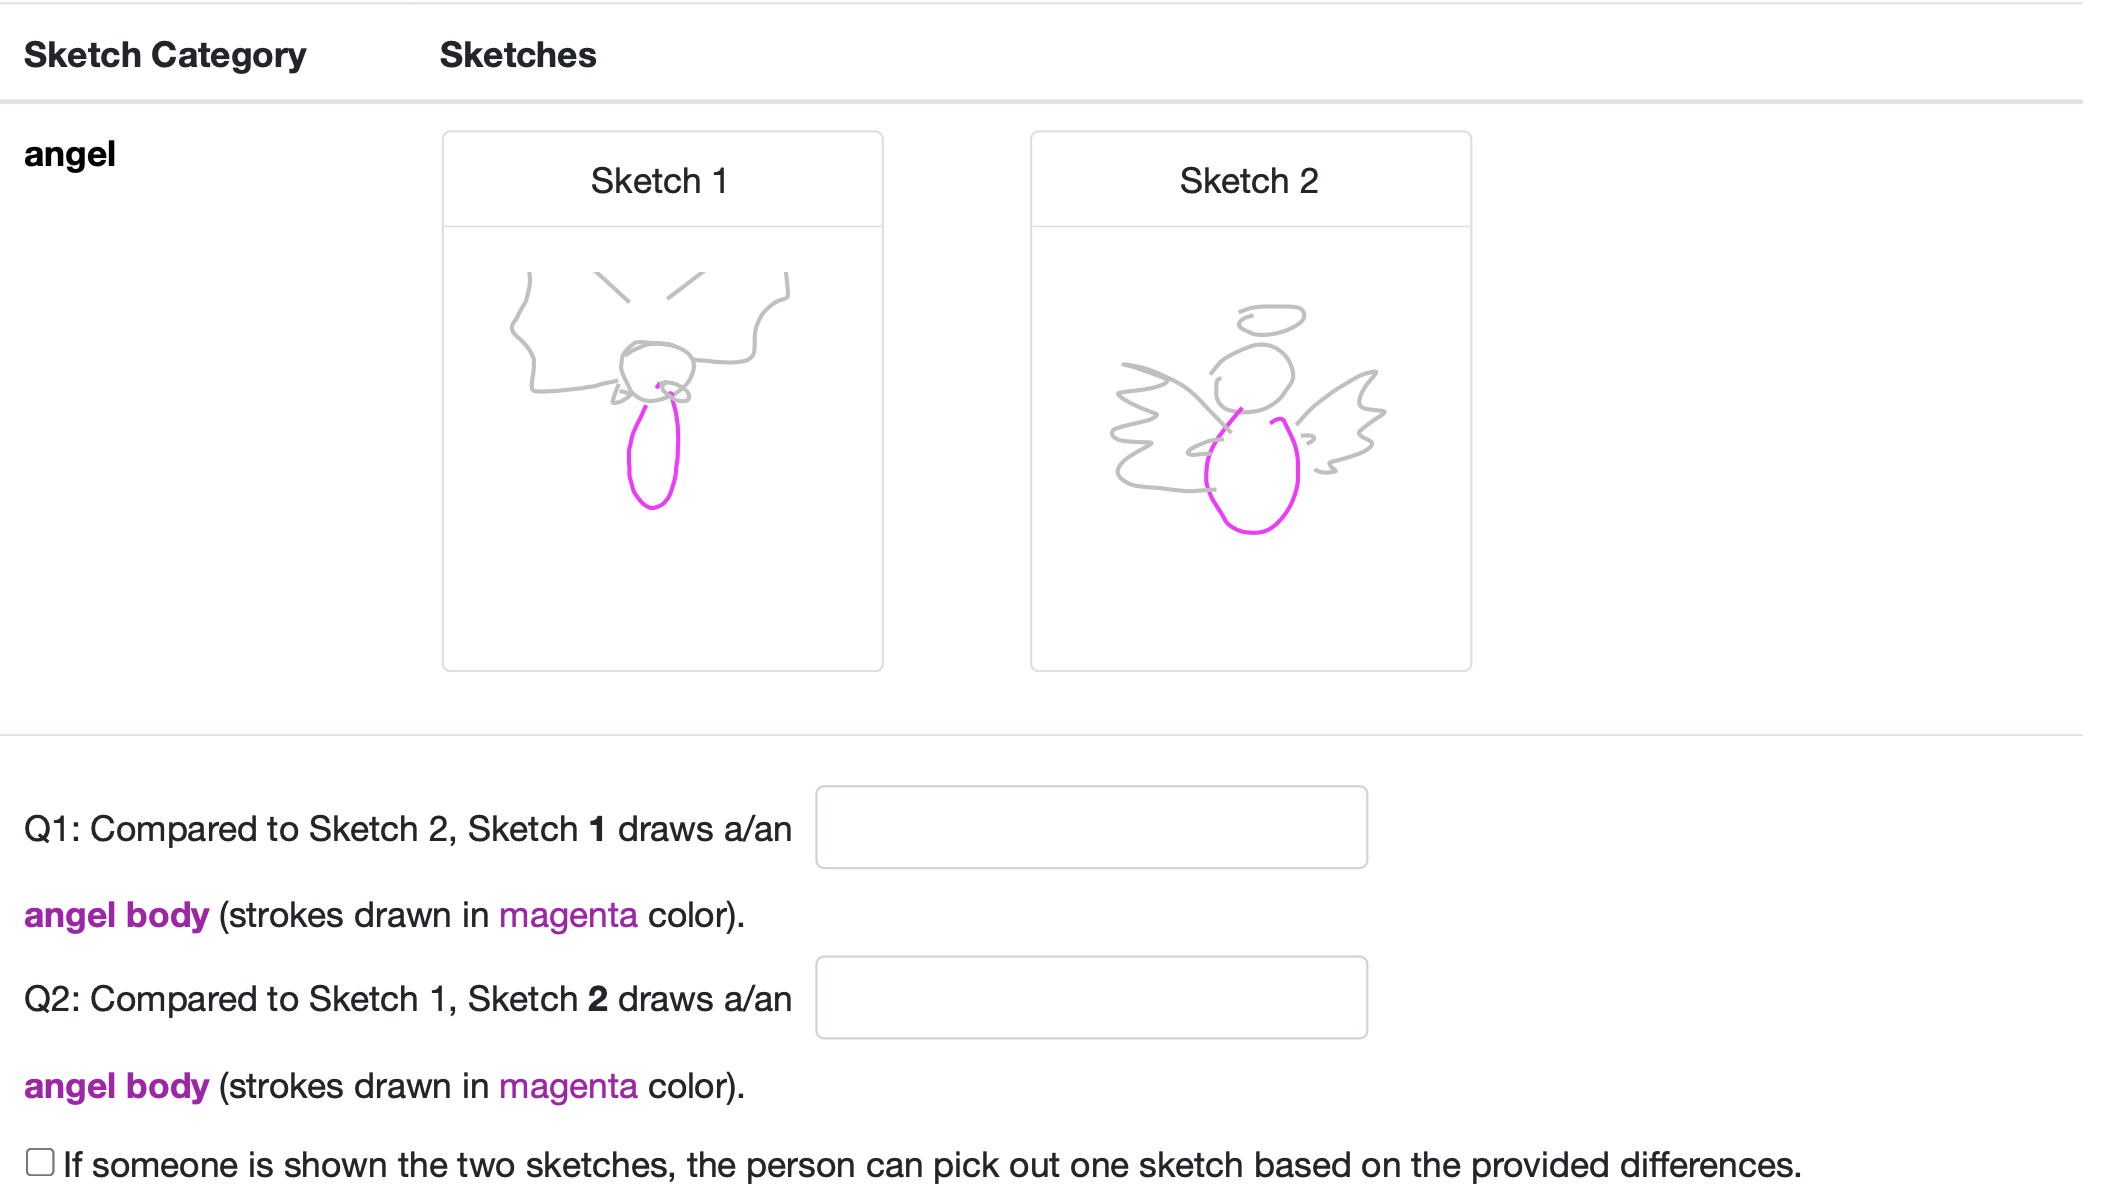
\includegraphics[width=.8\linewidth]{data_collection/pilot_02_04_annotation.png}  
  \caption{Design of main task for second pilot.}
  \label{v2.main_task.1.b}
\end{subfigure}
\end{figure*}

\begin{figure*}[ht!]
\ContinuedFloat
\begin{subfigure}{\textwidth}
  \centering
  % include third image
  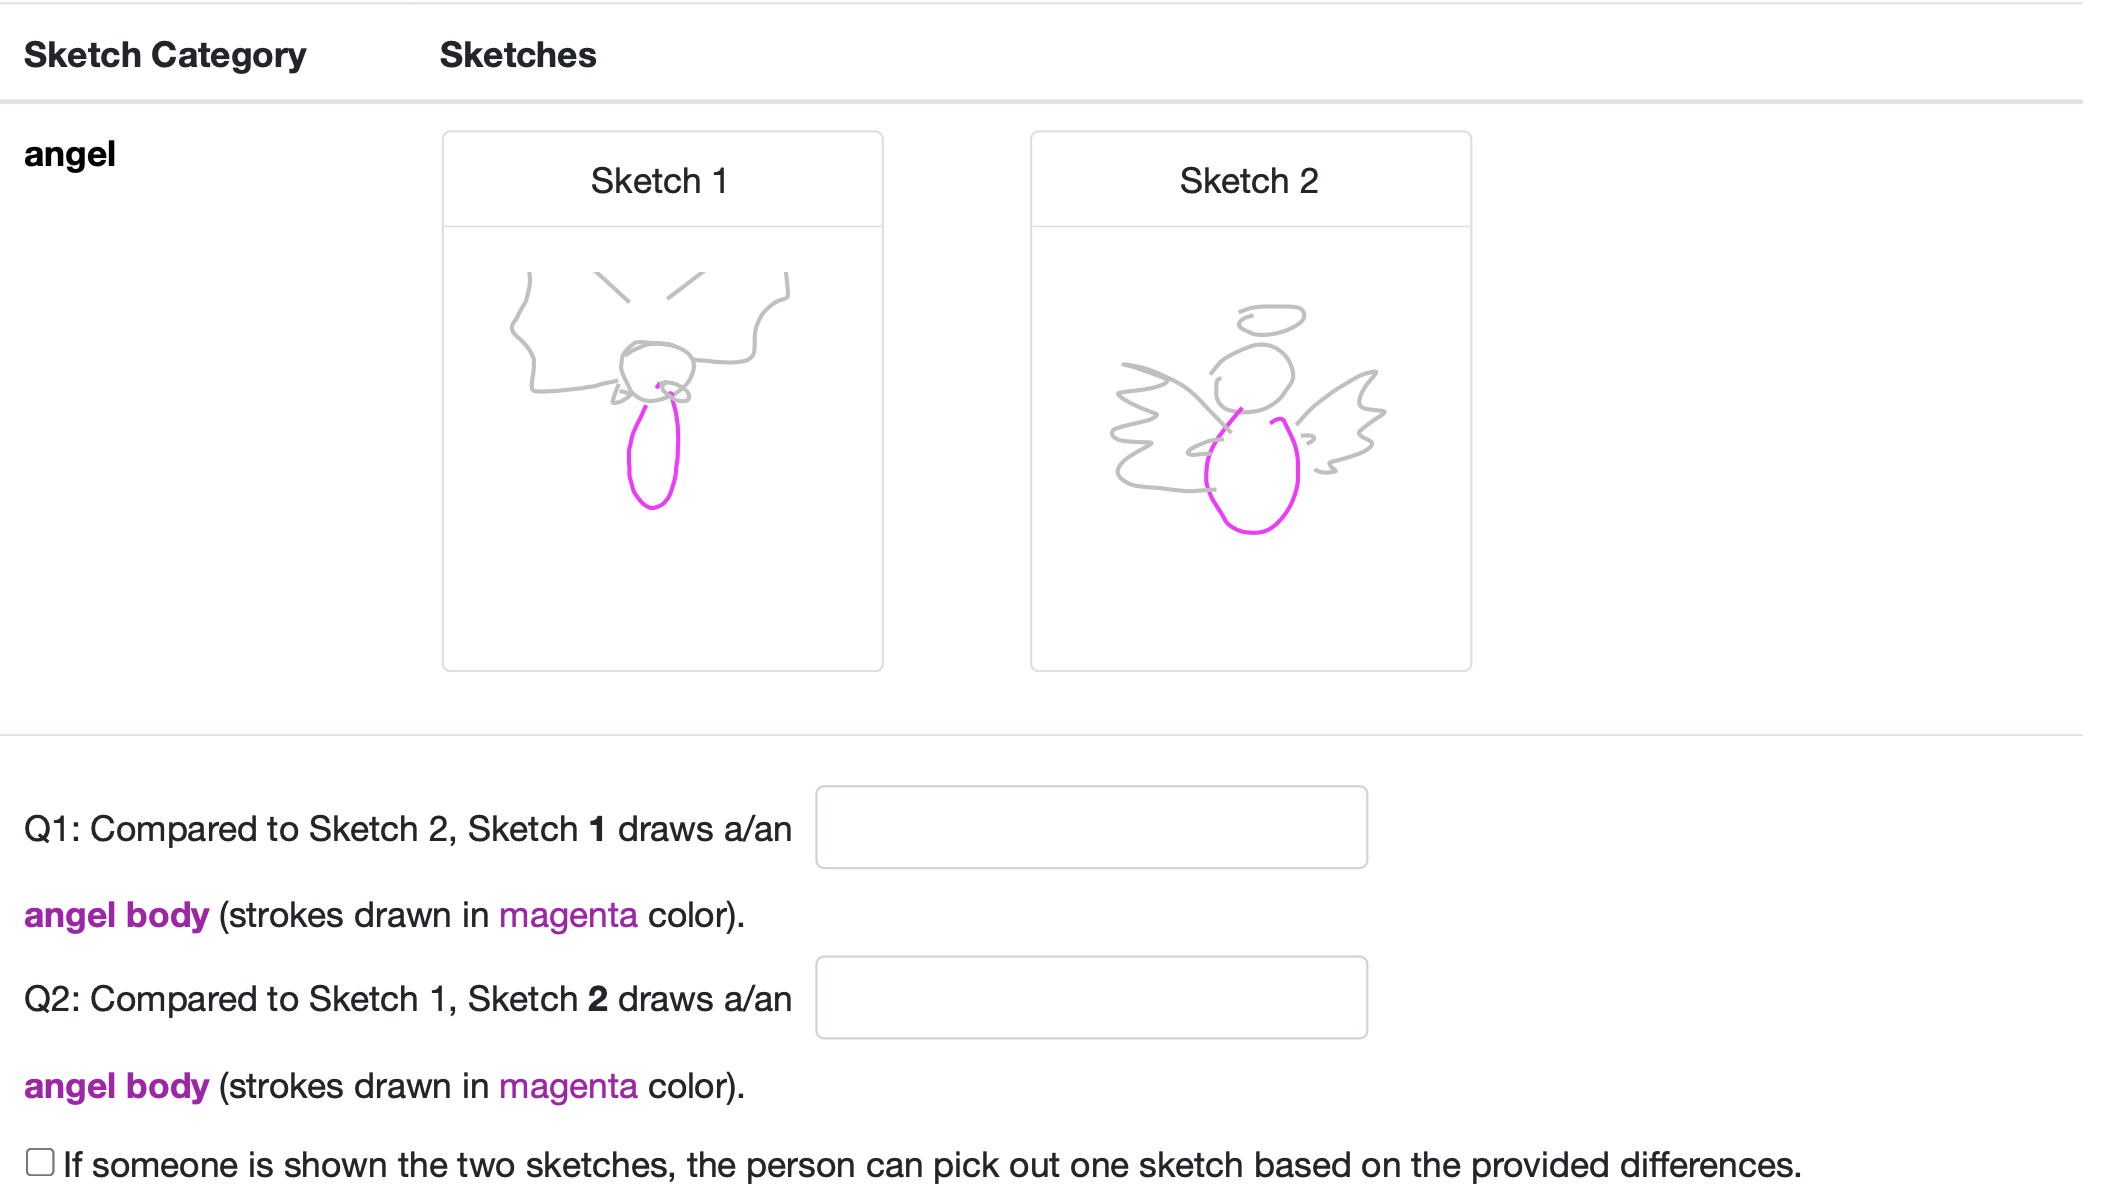
\includegraphics[width=.8\linewidth]{data_collection/pilot_02_04_annotation.png}  
  \caption{Design of main task for third pilot.}
  \label{v2.main_task.1.c}
\end{subfigure}
\newline
\begin{subfigure}{\textwidth}
  \centering
  % include third image
  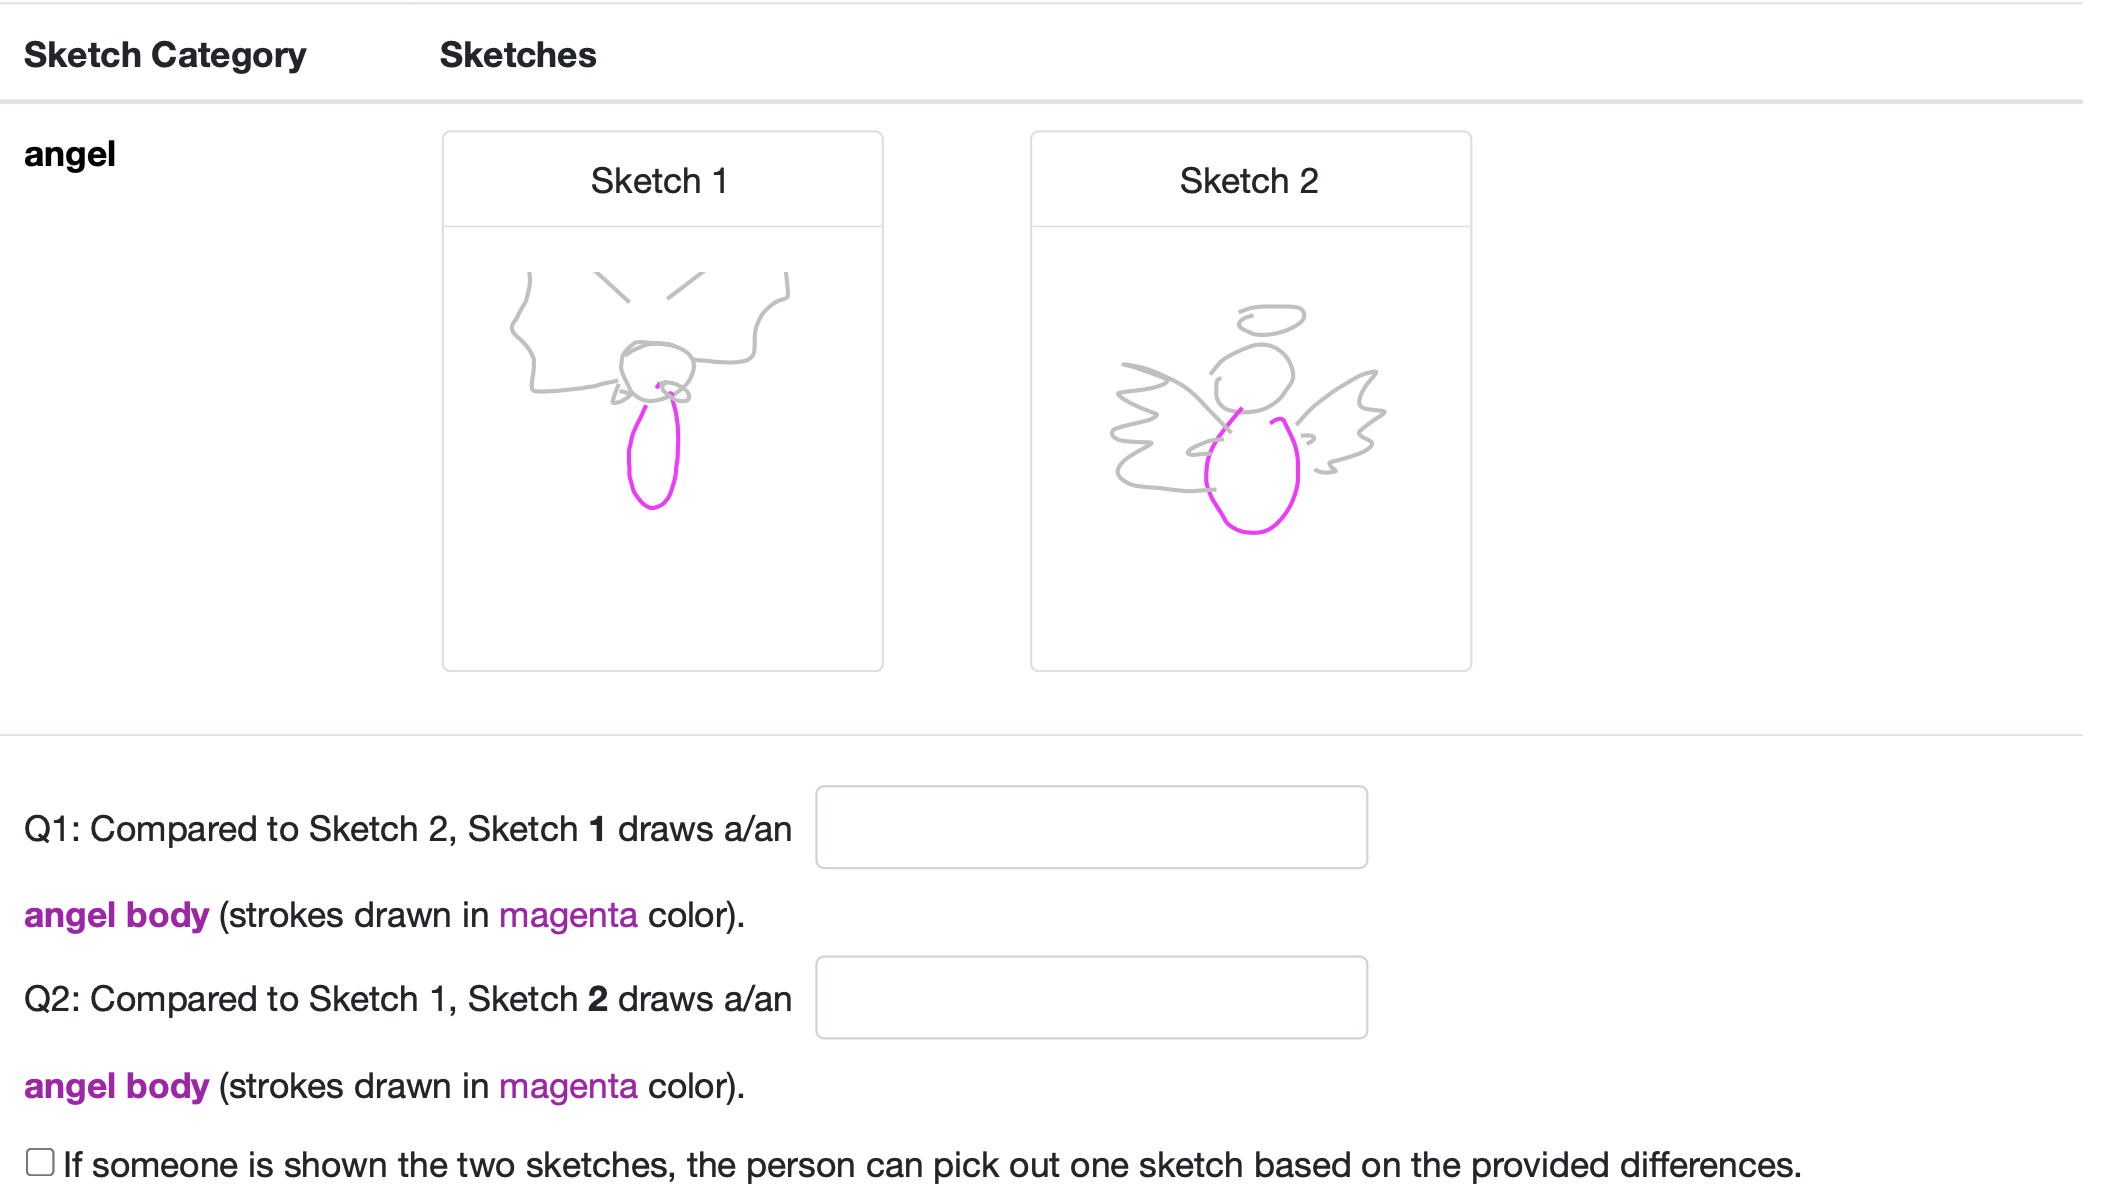
\includegraphics[width=.8\linewidth]{data_collection/pilot_02_04_annotation.png}  
  \caption{Design of main task for final task.}
  \label{v2.main_task.1.d}
\end{subfigure}
\caption{Progress of the design two for the main task in version two.}
\label{v2.main_task.1}
\end{figure*}

\subsubsection{Instructions}
At first the set of instructions was very restrictive and limit the annotators to pay attention to three types of differences: shapes, size relative to other objects in the same sketch, position relative to other objects in the same sketch. The general trend of the changes to the instructions is that we only require that the annotators fill in the blank with adjective phrases and try to not put too much restrictions on the language, in order to achieve our goal of building a dataset with free-form language instructions. 

In this version, the advantage is that since we have greatly simplify the task to only providing the textual descriptions, the turkers do not have to spend time coming up with drawings for a \textit{adjective}$\times$\textit{noun} prompt, and they do not have to put effort into keeping track of their drawing process to decide how to divide the drawing process into steps and then annotate for each step. Essentially, they only have to do the last step. Therefore, the requirements are much easier to write, and we do not have to specify anything in terms of providing drawings that correspond well with the prompts and providing annotations that align well with the drawings in the each step. 
One thing we tried was to somewhat rely on the examples to give an idea of what kind of annotations we want. Some examples that we used in the tasks are shown in Figure .
However, the downside for doing so is that the vocabularies used in by the annotators are primed by those in the examples, and we see that annotators would tend to repeat these vocabularies. Therefore, we especially added the requirement that states the annotators are not limited to words used in the examples, and they should use any words that can illustrate the parts well. The full set of requirements used in the final version is shown in Figure \ref{v2.requirement.1}.

\begin{figure*}[h]
\begin{subfigure}{0.5\textwidth}
  \centering
  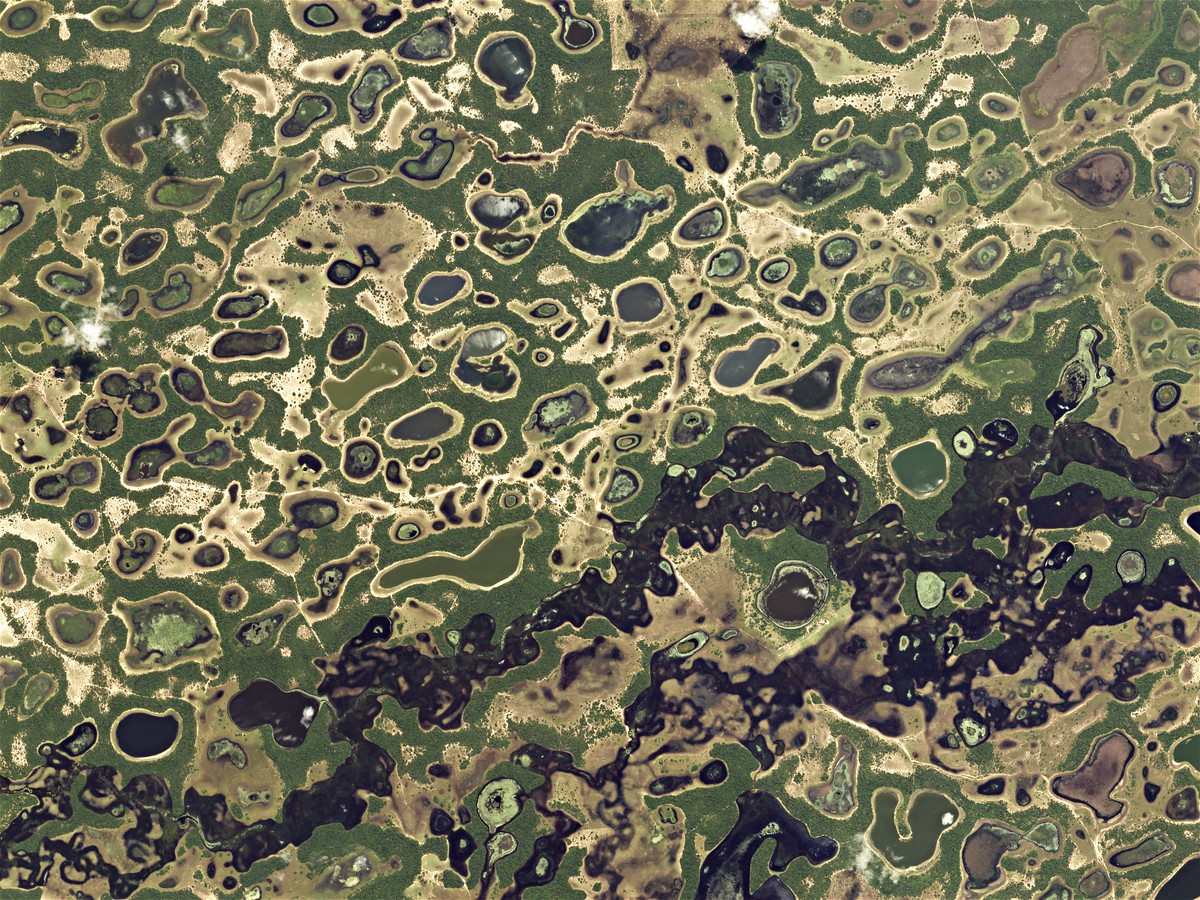
\includegraphics[width=.8\linewidth]{pantanal.jpeg}  
  \caption{Design of main task for first pilot.}
  \label{v2.requirement.examples.1}
\end{subfigure}
\begin{subfigure}{0.5\textwidth}
  \centering
  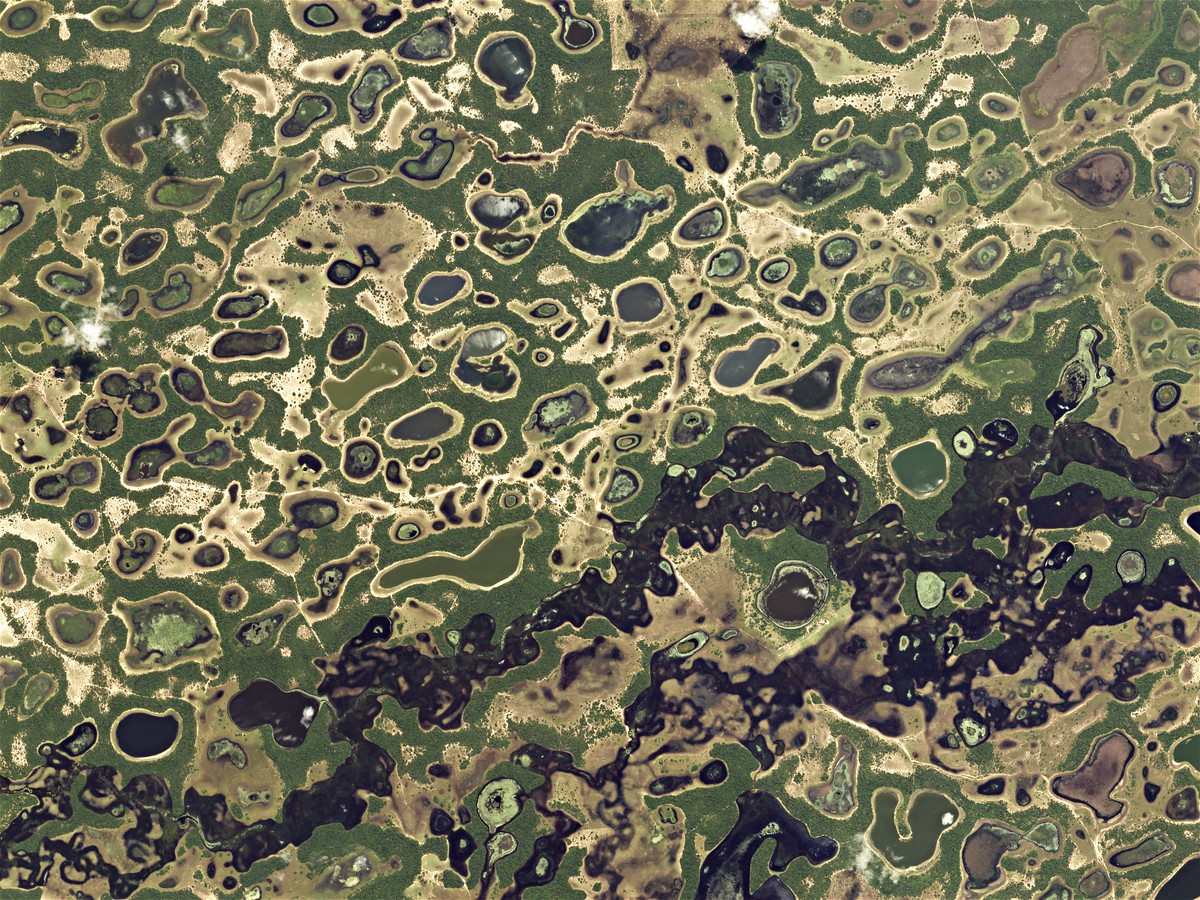
\includegraphics[width=.8\linewidth]{pantanal.jpeg}  
  \caption{Design of main task for first pilot.}
  \label{v2.requirement.examples.2}
\end{subfigure}
\newline
\begin{subfigure}{0.5\textwidth}
  \centering
  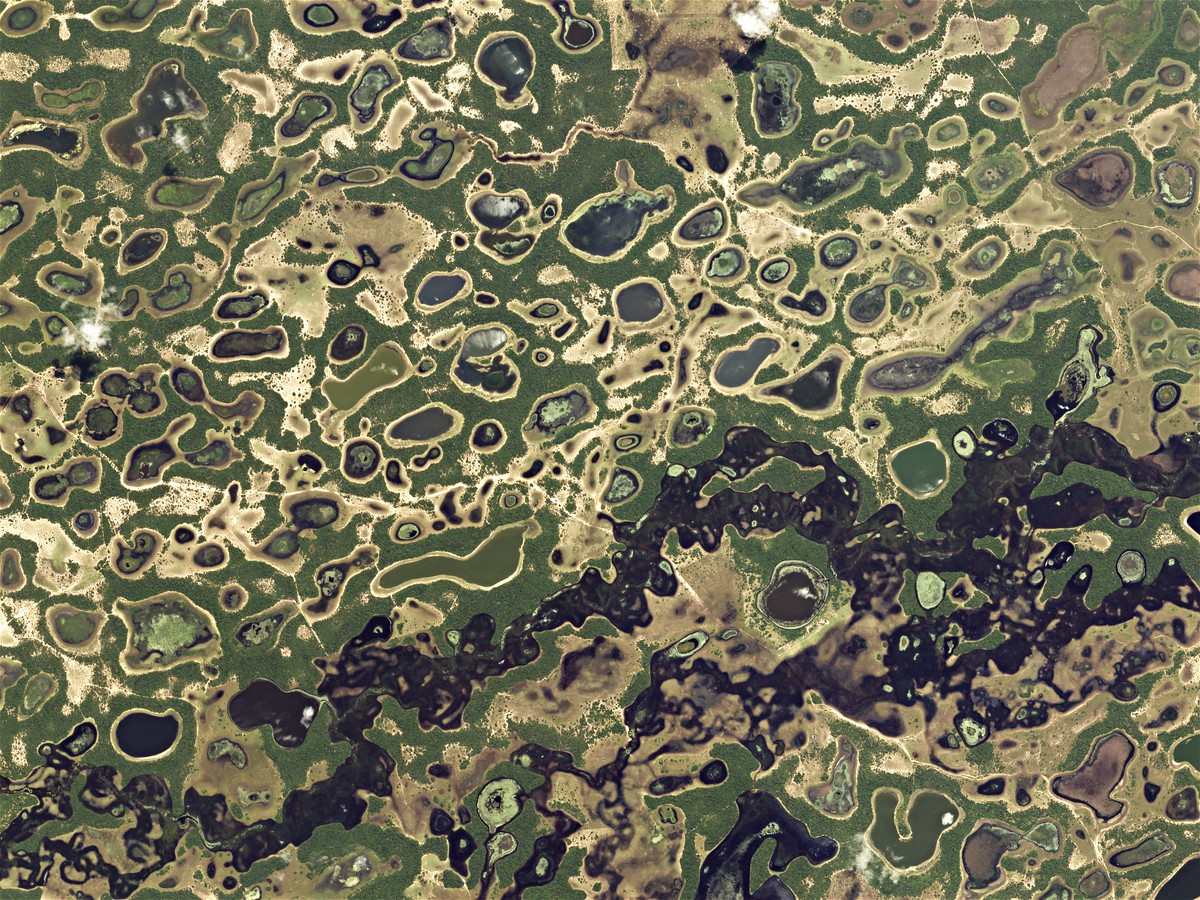
\includegraphics[width=.8\linewidth]{pantanal.jpeg}  
  \caption{Design of main task for second pilot.}
  \label{v2.requirement.examples.3}
\end{subfigure}
\begin{subfigure}{0.5\textwidth}
  \centering
  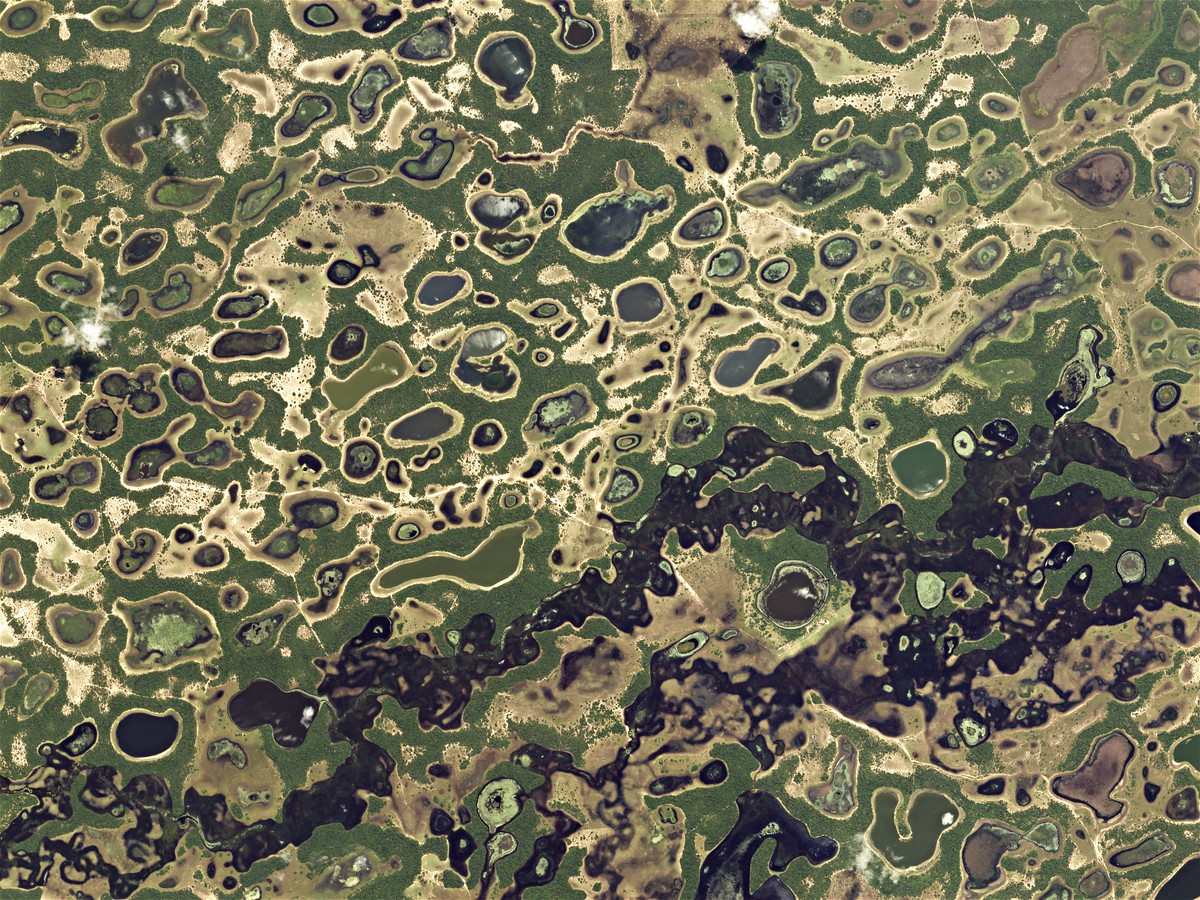
\includegraphics[width=.8\linewidth]{pantanal.jpeg}  
  \caption{Design of main task for second pilot.}
  \label{v2.requirement.examples.4}
\end{subfigure}
\newline
\begin{subfigure}{0.5\textwidth}
  \centering
  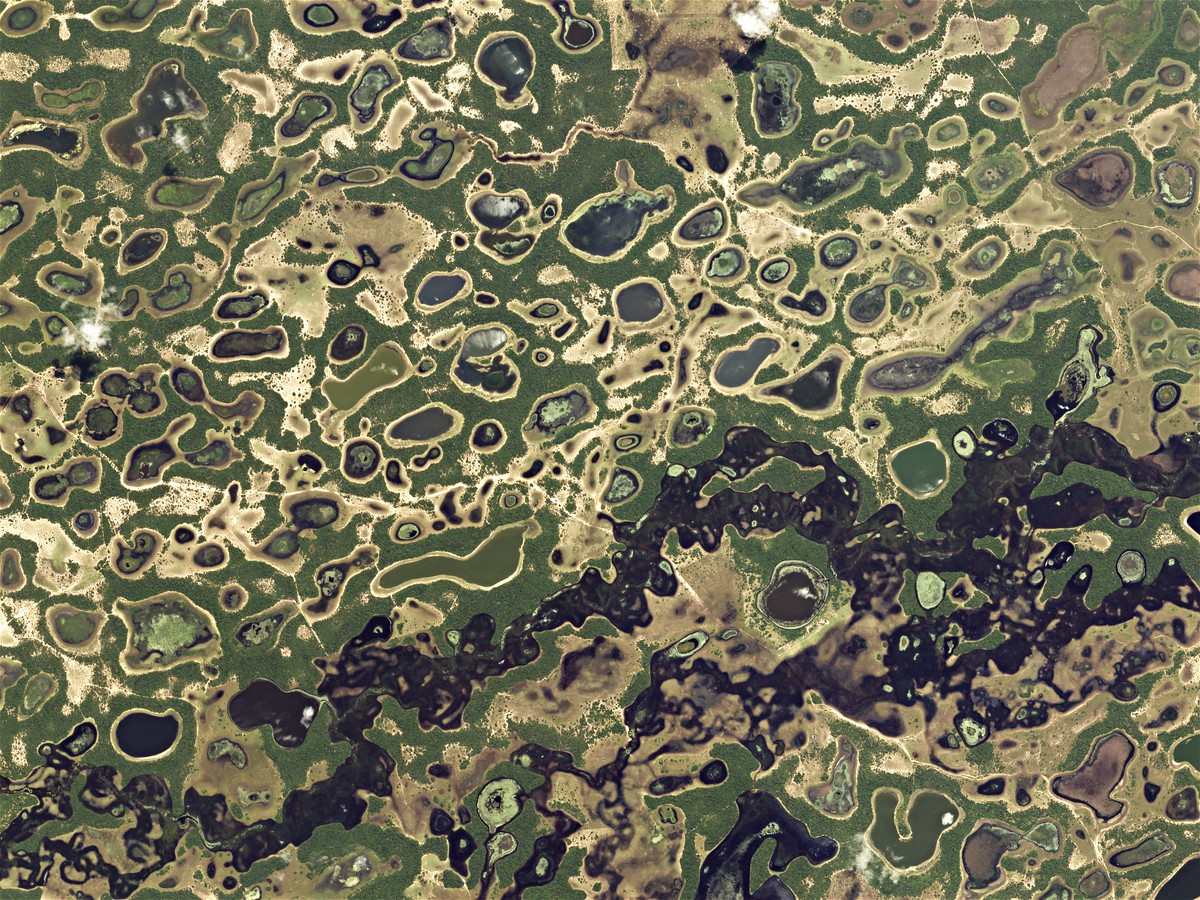
\includegraphics[width=.8\linewidth]{pantanal.jpeg}  
  \caption{Design of main task for second pilot.}
  \label{v2.requirement.examples.5}
\end{subfigure}
\begin{subfigure}{0.5\textwidth}
  \centering
  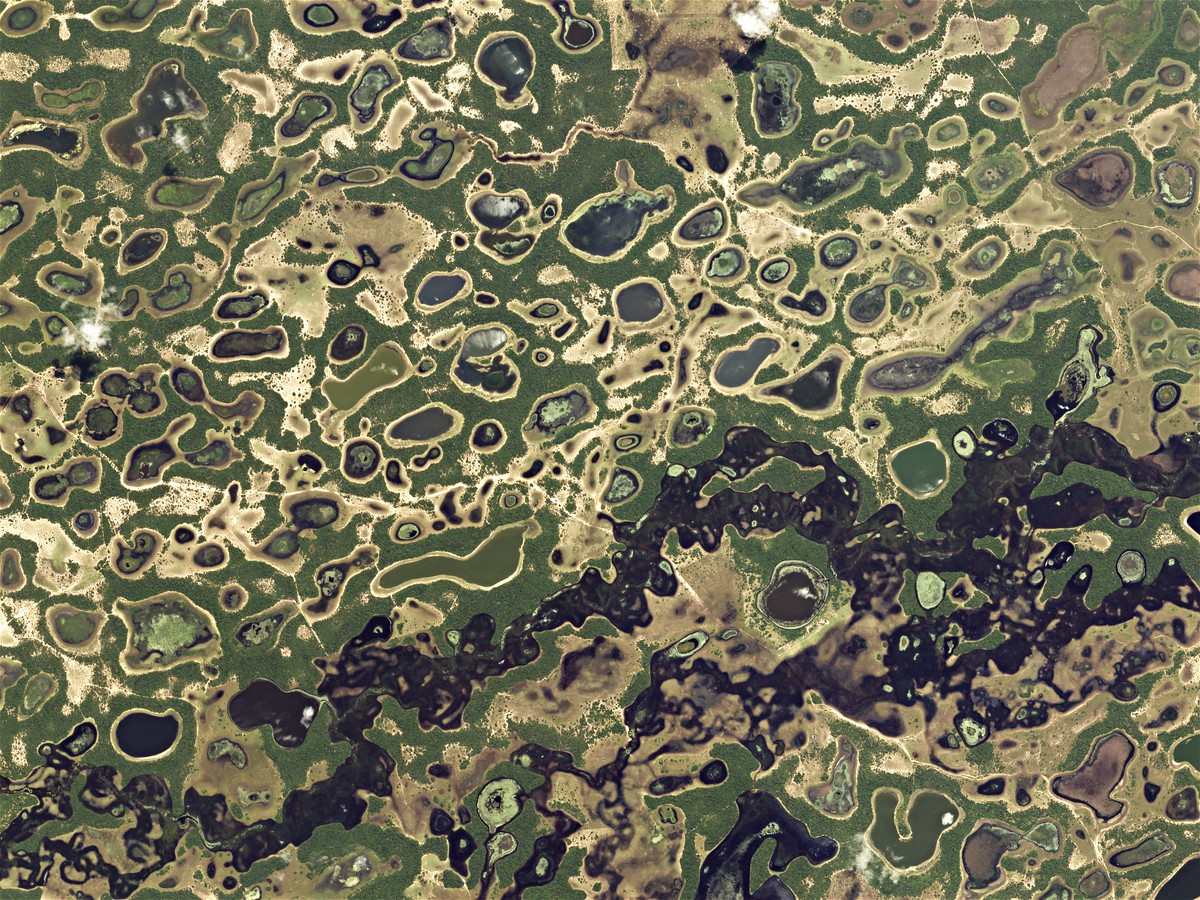
\includegraphics[width=.8\linewidth]{pantanal.jpeg}  
  \caption{Design of main task for second pilot.}
  \label{v2.requirement.examples.6}
\end{subfigure}
\caption{Progress of the design two for the main task in version two.}
\label{v2.requirement.examples}
\end{figure*}

\begin{figure*}[h]
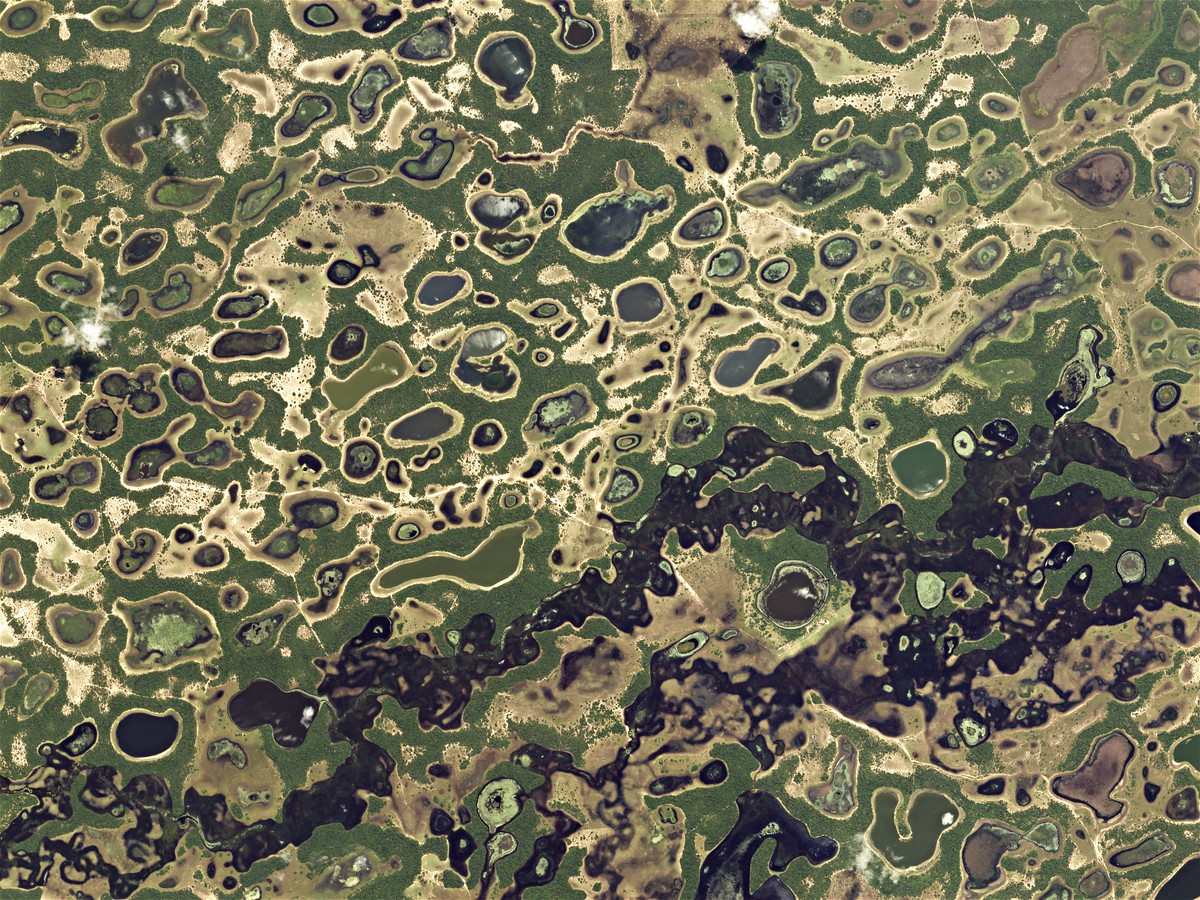
\includegraphics[width=.8\linewidth]{pantanal.jpeg}  
\caption{The set of requirements used in the final task.}
\label{v2.requirement.1}
\end{figure*}

The requirement that was a bit challenging for people to understand was the one regarding
\textit{Do not use adjectives related to personal opinions, such as random, good, messy, beautiful, and strage, that are hard to achieve consensus if others were to validate your answers.}. Since we hope that the model can get signal from the texts about what kind of figures to draw, words that do not directly convey visual properties of the parts are not helpful. We later changed the wording to \textit{Do not use adjectives that fail to describe specific visual properties of the objects in the sketches}. A slight caveat here is that we actually hope to collect descriptions that describe the emotions expressed in the sketches. We know beforehand that we hope to collect a dataset for the \textit{face} category, so it is quite common for faces to express emotions like happy and sad, and we were slightly worried that some turkers might consider these words as not illustrating enough visual properties about the drawings, since they are quite abstract, at least compared to adjectives like \textit{rectangular} or \textit{wide}. 

\subsubsection{Qualifications}
We prepared 10 qualification questions, all in the style of yes/no questions. We will use the qualification test to filter annotators who have read through all the instructions and examples and have formed a good understanding of the task. The 10 questions are shown in Figure \ref{v2.qualification.1}. We provides hints in each questions that explicitly state which requirement and examples are helpful for solving the questions. The purpose of the qualification test is not to trick annotators but to ensure both quality and speed of the annotations. 

\begin{figure*}[h]
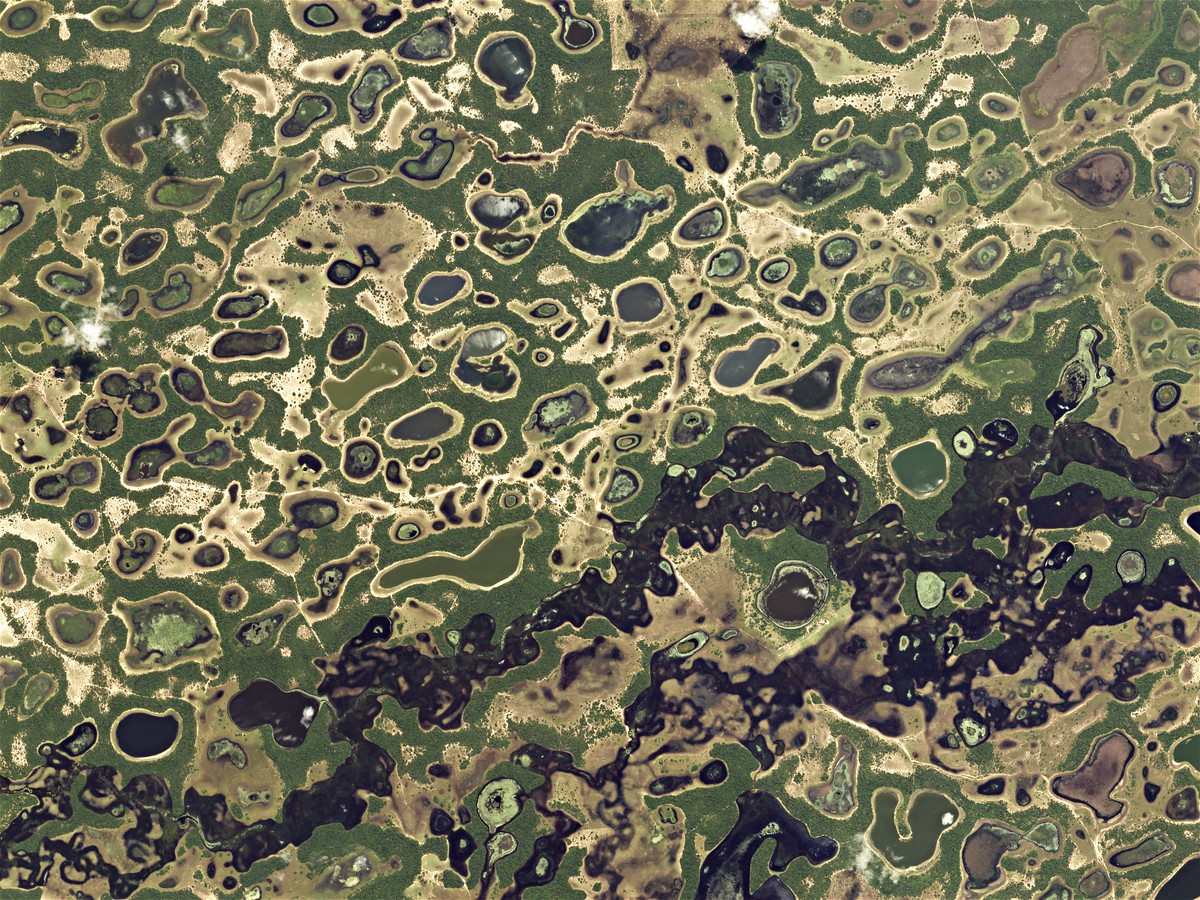
\includegraphics[width=.8\linewidth]{pantanal.jpeg}  
\caption{The qualification questions.}
\label{v2.qualification.1}
\end{figure*}

We released $n$ copies of qualifications, and $n_2$ annotators scored $90$ or higher. The average score for the entire test is $x$, and the rate of correct answer for each question is shown in Table \ref{v2.qualification.success_rate}. Before releasing the qualification, we have tested the test on 
\begin{table*}[h!]
\begin{minipage}[b]{1\textwidth}
\centering
\begin{tabular}{l|rrrrrrrrrr}
\toprule
Question Number  & 1 & 2 & 2 & 2 & 2 & 2 & 2 & 2 & 2 & 2  \\
Correct Rate  & 1 & 2 & 2 & 2 & 2 & 2 & 2 & 2 & 2 & 2\\
\bottomrule
\end{tabular}
\caption{Success rate of each question in the qualification test}
\label{v2.qualification.success_rate}
\end{minipage}
\end{table*}

\subsection{Results}

\subsubsection{Pilot 1}
In order to work out the data collection process, we chose the angel category and try to manually examine the sketches and categorize them based on 


One purpose of the pilot is to estimate the amount of money that we need to spend for each task, and from Table \ref{v2.workertime}, we see that []
\begin{table*}[h!]
\begin{minipage}[b]{1\textwidth}
\centering
\begin{tabular}{l|rrrrr}
\toprule
~ & Max. & Min. & Mean & Med. & Std. \\
\midrule
Feb 01 Pilot  & 1 & 2 & 2 & 2 & 2   \\
Feb 04 Pilot  & 1 & 2 & 2 & 2 & 2  \\
Feb 08 Pilot  & 1 & 2 & 2 & 2 & 2  \\
Official Collection  & 1 & 2 & 2 & 2 & 2  \\
\bottomrule
\end{tabular}
\caption{Comparing time statistics of pilot task}
\label{v2.workertime}
\end{minipage}
\end{table*}

For the data collection process, we decide to collect for the face category of the QuickDraw dataset, and the reason for it was mainly to echo the choice of many SOTA generative modeling works that are done on the CelebA dataset. It seems that face generation is quite a starting point for many of the generative modeling work. We have also surveyed some text-to-image synthesis methods that use datasets like (1) CUB dataset (2) MNIST (3) Omniglot. Several sketch datasets include the one from DoodlerGAN and SketchBirds. A lot of the datasets focus on one or two categories, so we decide to do the same to ensure that with our budge, we can collect a dataset that contains enough signal to train a generative ML model. 

Clustering the faces, we strive to present to the annotators pairs of faces that are distinct as possible in order help them to provide good annotations. It is easier for them to grasp and understand the features of the objects if two sketches are presented in a contrasting way. 



If we use CLIP to extract the visual features for the entire face sketch.



The heuristic that we use to choose how to pair up